\documentclass[a4paper]{article}

\usepackage[12pt]{extsizes}

\usepackage{mathtext}

\usepackage[T2A]{fontenc}
\usepackage[utf8]{inputenc}

\usepackage[english,russian]{babel}

\usepackage{indentfirst}
\usepackage{scrextend}
\usepackage{fancyhdr}
\newcommand*\rot{\rotatebox{90}}

\usepackage{xr}
\usepackage{verbatimbox}
\usepackage{caption}
\usepackage{graphicx}

\usepackage{gensymb}
\usepackage{tabu}

\usepackage{listings}
\usepackage{color}
\definecolor{mygreen}{rgb}{0,0.6,0}
\definecolor{mygray}{rgb}{0.5,0.5,0.5}
\lstset{extendedchars=\true,
		breaklines=true,
		breakatwhitespace=true,
		captionpos=b,
		keepspaces=true,
		keywordstyle=\color{blue},
		numbers=left,
		tabsize=4,
		numberstyle=\tiny\color{mygray},
		commentstyle=\color{mygreen},
		language=C,
		basicstyle=\ttfamily,
		showstringspaces=false,
		title=\lstname
		}
 
\usepackage{geometry} % Меняем поля страницы
\geometry{left=2.8cm}% левое поле
\geometry{right=2.8cm}% правое поле
\geometry{top=2.5cm}% верхнее поле
\geometry{bottom=3cm}% нижнее поле

\usepackage{perpage}
\usepackage{placeins} % for float barriers
\usepackage{float}
\MakePerPage{footnote}

\setcounter{tocdepth}{2}
\ifx
Выставление глубины оглавления
n=4 это chapter, section, subsection, subsubsection и paragraph;
n=3 это chapter, section, subsection и subsubsection;
n=2 это chapter, section, и subsection;
n=1 это chapter и section;
n=0 это chapter.
\fi

\renewcommand*\thesection{\arabic{section}.}
\renewcommand{\thesubsection}{\thesection\arabic{subsection}}
\renewcommand{\thetable}{\thesection\arabic{table}}
\renewcommand{\theequation}{\thesection\arabic{equation}}

\newcommand{\newpar}{\par\medskip}
\usepackage{multirow,tabularx}

\newcommand{\sbt}{
	\,\begin{picture}(-1,1)(-1,-3)\circle*{4}\end{picture}\ 
}
\newcommand{\sbti}{\sbt~~}

\newcommand{\linux}{Linux}
\newcommand{\linuxv}{\linux\ v.3.9.2\ }
\newcommand{\gnu}{GNU}
\newcommand{\gnulinux}{\gnu/\linux}
\newcommand{\archlinux}{Arch Linux}
\newcommand{\fulllinux}{\archlinux, ядро \linuxv}
\newcommand{\unix}{UNIX\ }

\newcommand{\linuxpath}[1]{\texttt{#1}}
\newcommand{\linuxutil}[1]{\texttt{#1}}
\newcommand{\linuxcommand}[1]{\texttt{#1}}
\newcommand{\src}[1]{\linuxcommand{#1}}
\newcommand{\key}[1]{\src{<#1>}}

\begin{document}
	\thispagestyle{fancy}

\fancyhead[C]{
	Федеральное государственное бюджетное 
	образовательное учреждение высшего 
	профессионального образования\\
	<<Московский государственный технический 
	университет им.~Н.\,Э.~Баумана>>
}
\fancyfoot[C]{ Москва, 2014г. }

\vspace*{2cm}

\begin{flushright}
	\Large{ Факультет: }\\
	\large{ <<Информатика и системы управления>> }\\
	\Large{ Кафедра: }\\
	\large{ <<Программное обеспечение ЭВМ и\\ 
		информационные технологии>> }
\end{flushright}

\vspace{2cm}

\begin{LARGE} 
	\begin{center} 
		Расчетно\,--\,пояснительная записка\\
		к дипломному проекту по теме\\ 
		\vspace{2cm}
        Распознавание человеческого лица по фотоснимку на мобильной
        платформе под управлением ОС Android
	\end{center}
\end{LARGE}

\vspace{5cm}

\begin{flushright}
	\begin{tabular}{ll}
	Руководитель дипломного проекта:&Майков~К.\,А.\\
	Исполнитель дипломного проекта:&Бережной~П.\,Ю.
	\end{tabular}
\end{flushright}

\newpage
\setcounter{page}{1}

	\tableofcontents
    \newpage
    \section{Организационно-экономическая часть}

В данном разделе будет проведен расчет трудоемкости выполнения работ, расчет количества исполнителей,
построение календарного плана, расчет конечной стоимости и экономической эффективности программного продукта (ПП).

\subsection{Введение}

Заказчиком (кафедрой) сформулировано техническое задание на разработку ПП.

Необходимо разработать ПП, осуществляющий распознавание лиц в реальном
времени с приемлемой точностью.

Данный проект выполнен в среде Emacs.
Заказчик предполагает реализовывать ПП на электронном информационном
носителе (компакт-диске).

На рынке подобные продукты представлены как
бесплатными продуктами (OpenCv, PCL), так и коммерческими продуктами (Синезис).

Расчёты производились в соответствии с \cite{econ_1}.

\subsubsection{Организация и планирование процесса разработки}

При использовании традиционного подхода, организация и планирование
процесса разработки программного продукта или программного комплекса
предусматривает выполнение следующих работ:
\begin{itemize}
	\item формирование состава выполняемых работ и группировка их по
	стадиям разработки;
	\item расчет трудоемкости выполнения работ;
	\item установление профессионального состава и расчет количества
	исполнителей;
	\item определение продолжительности выполнения отдельных этапов разработки;
	\item построение календарного графика выполнения разработки;
\end{itemize}

Планирование длительности этапов и содержания проекта осуществляется в
соответствии с ЕСПД ГОСТ 34.603-92 и распределяет работы по этапам,
как показано в таблице~\ref{table:econ_1}.
\begin{table}[ht]
    \centering
	\begin{tabu}[\textwidth]{|c|c|l|}
		\hline
		Основные стадии & № & Содержание работы \\
		\hline
		\multirow{2}{*}{Техническое задание}
			& 1 & Постановка задачи\\
			\cline{2-3}
			& 2 & Выбор средств разработки и реализации\\
		\hline
		\multirow{2}{*}{Эскизный проект}
			& 3 & Разработка математической модели\\
			\cline{2-3}
			& 4 & Разработка алгоритмов расчёта задачи\\
		\hline
		\multirow{3}{*}{Техно-рабочий проект}
			& 5 & Реализация алгоритмов расчёта задачи\\
			\cline{2-3}
			& 6 & Разработка пользовательского интерфейса\\
			\cline{2-3}
			& 7 & Реализация пользовательского интерфейса\\
		\hline
		Внедрение & 8 & Проведение вычислительных экспериментов\\
		\hline
	\end{tabu}
	\captionsetup{justification=centering}
	\caption{Распределение работ по этапам.}
	\label{table:econ_1}
\end{table}

\subsubsection{Расчёт трудоёмкости выполнения работ}

Трудоемкость разработки программной продукции зависит от ряда факторов,
основными из которых являются следующие:
\begin{itemize}
	\item степень новизны разрабатываемого программного комплекса,
	\item сложность алгоритма его функционирования,
	\item объем используемой информации, вид ее представления и способ
	обработки,
	\item уровень используемого алгоритмического языка программирования
\end{itemize}

Исходные данные расчета приведены в таблице~\ref{table:econ_2}
\begin{table}[ht]
    \centering
	\begin{tabu}[\textwidth]{|X[l]|X[l]|}
		\hline
		Функциональное назначение ПП & Управление лицензиями на
		программное обеспечение в техническом университете.\\
		\hline
		Степень новизны разрабатываемого проекта & Группа новизны
		\texttt{B} - разработка программной продукции, имеющей
		аналоги.\\
		\hline
		Степень сложности алгоритма функционирования & \texttt{3}
		группа сложности - программная продукция, реализующая
		алгоритмы стандартных методов решения задач. \\
		\hline
		По виду представления исходной информации & Группа \texttt{12}
		- исходная информация представлена в форме докуметов, имеющих
		одинаковый формат и структуру, требуется форматный контроль
		информации. \\
		\hline
		Структура выходным документов & Группа \texttt{22} - требуется
		вывод на печать одинаковых документов, вывод информационных
		массивов на машинные носители.\\
		\hline
	\end{tabu}
	\captionsetup{justification=centering}
	\caption{Исходные данные}
	\label{table:econ_2}
\end{table}

Трудоемкость разработки программной продукции $\tau_{ПП}$ может быть определена
как сумма величин трудоемкости выполнения отдельных стадий разработки
ПП из выражения:
\begin{equation}
	\tau_{ПП} = \tau_{ТЗ} + \tau_{ЭП} + \tau_{ТП} + \tau_{РП} + \tau_{В}
\label{F:econ_1}
\end{equation}
где
\begin{itemize}
	\item $\tau_{ТЗ}$ - трудоемкость разработки технического задания на
	создание ПП;
	\item $\tau_{ЭП}$ - трудоемкость разработки эскизного проекта ПП;
	\item $\tau_{ТП}$ - трудоемкость разработки технического проекта ПП;
	\item $\tau_{РП}$ - трудоемкость разработки рабочего проекта ПП;
	\item $\tau_{В}$ - трудоемкость внедрения разработанного ПП.
\end{itemize}

Трудоемкость разработки технического задания рассчитывается по формуле:
\begin{equation}
	\tau_{ТЗ} = T_{ЗРЗ} + T_{ЗРП}
\label{F:econ_2}
\end{equation}
где
\begin{itemize}
	\item $T_{ЗРЗ}$ - затраты времени разработчика постановки задач на
		разработку ТЗ, чел. дни;
	\item $T_{ЗРП}$ - затраты времени разработчика программного
		обеспечения на разработку ТЗ, чел. дни.
\end{itemize}

В расчёте участвуют следующие коэффициенты:
\begin{itemize}
	\item $t_{З} = 47$ -- норма времени на разработку ТЗ на программный
		продукт в зависимости от функционального назначения и степени новизны
		разрабатываемого ПП, чел. дни;
	\item $K_{ЗРЗ} = 0,65$ -- коэффициент, учитывающий удельный вес
		трудоемкости работ, выполняемых разработчиком постановки на стадии ТЗ;
	\item $K_{ЗРП} = 0,35$ -- коэффициент, учитывающий удельный вес
		трудоемкости работ, выполняемых разработчиком программного обеспечения
		на стадии ТЗ.
\end{itemize}

Тогда
\begin{equation}
	\tau_{ТЗ} = 47 \cdot (0,65 + 0,35) = 47 [чел. дни]
\label{F:econ_3}
\end{equation}

Аналогично рассчитывается трудоёмкость эскизного проекта ПП $\tau_{ЭП}$:
\begin{equation}
	\tau_{ЭП} = t_{ЭП} \cdot (K_{ЭРЗ} + K_{ЭРП}) = 67 \cdot (0,75 + 0,25) = 67 [чел. дни]
\label{F:econ_4}
\end{equation}

Трудоемкость разработки технического проекта $\tau_{ТП}$ зависит от функционального
назначения ПП, количества разновидностей форм входной и выходной информации
и определяется как сумма времени, затраченного разработчиком постановки
задач и разработчиком программного обеспечения, т.е.
$$\tau_{ТП} = (t_{ТРЗ} + t_{ТРП}) \cdot К_{В} \cdot К_{р}$$
$$К_{В} = (К_{П} n_{П} + К_{НС} n_{НС} + К_{Б} n_{Б} )/(n_{П} + n_{НС} + n_{Б})$$
где
\begin{itemize}
	\item $t_{ТРЗ} = 57, t_{ТРП} = 43$ - норма времени, затрачиваемого на
		разработку технического проекта разработчиком постановки задач и
		разработчиком ПП соответственно, чел.-дни
	\item $K_{p} = 1,26$ - коэффициент учета режима обработки информации
	\item $К_{П} = 1, К_{Н}С = 0,72, К_{Б} = 2, 18$ - значения
		коэффициентов учета вида используемой информации для переменной,
		нормативно-справочной информации и баз данных соответственно
	\item $n_{П} = 6, n_{Н}С = 4, n_{Б} = 0$ - значения коэффициентов
		учета вида используемой информации для переменной,
		нормативно-справочной информации и баз данных соответственно
\end{itemize}

Тогда
$$\tau_{ТП} = (57 + 43)(1 \cdot 6 + 0,72 \cdot 4 + 2,18 \cdot 0)/(6 + 4 + 0)
\cdot 1,26 = 112 [чел. дни]$$

Трудоемкость разработки рабочего проекта $\tau_{РП}$ зависит от функционального
назначения ПП, количества разновидностей форм входной и выходной информации,
сложности алгоритма функционирования, сложности контроля информации,
степени использования готовых программных модулей, уровня алгоритмического
языка программирования и определяется по формуле:
$$\tau_{РП} = К_{к} К_{р} К_{Я} К_{З} К_{ИА} (t_{РРЗ} + t_{РРП})$$
$$K_{ИА} = (К^{'}_{П} \cdot n_{П} + К^{'}_{НС} \cdot n_{НС} + К^{'}_{Б} \cdot
n_{Б})/(n_{П} + n_{НС} + n_{Б} )$$

\begin{itemize}
	\item $t_{РРЗ} = 138, t_{РРП} = 979$ - норма времени, затраченного на
		разработку РП на алгоритмическом языке высокого уровня разработчиком
		постановки задач и разработчиком программного обеспечения соответственно,
		чел.дни.
	\item $K_{K} = 1$ - коэффициент учета сложности контроля информации;
	\item $K_{P} = 1,32$ - коэффициент учета режима обработки информации
	\item $K_{Я} = 1$ - коэффициент учета уровня используемого
		алгоритмического языка программирования;
	\item $K_{З} = 0,8$ - коэффициент учета степени использования готовых
		программных модулей;
	\item $K_{ИА}$ - коэффициент учета вида используемой информации и
		сложности алгоритма ПП;
	\item $К^{'}_{П} = 1,20, К_{Н}С^{'} = 0,65, К^{'}_{Б} = 0,54$ -
		значения коэффициентов учета сложности алгоритма ПП и вида
		используемой информации для переменной, нормативно-справочной
		информации и баз данных соответственно.
\end{itemize}

Тогда
$$К_{ИА} = 6 \cdot 1,20 + 4 \cdot 0,65/(4 + 6) = 0,98$$
$$\tau_{РП} = 1 \cdot 1,32 \cdot 1 \cdot 0,8 \cdot 0,98 \cdot (138 + 979) = 1117 [чел. дни]$$

Так как при разработке ПП стадии «Технический проект» и «Рабочий
проект» объединены в стадию «Техно-рабочий проект», то трудоемкость ее
выполнения $\tau_{ТРП}$ определяется по формуле
$$\tau_{ТРП} = 0,85\tau_{ТП} + \tau_{РП} = 0,85 \cdot 112 + 1117 = 1212 [чел. дни]$$

Трудоемкость выполнения стадии внедрения $\tau_{В}$ может быть рассчитана
по формуле:
$$\tau_{В} = К_{к} К_{р} К_{З} (t_{ВРЗ} + t_{ВРП} ) = 1 \cdot 1,32 \cdot 0,8(33 + 98) = 138 [чел.дни]$$

Трудоемкости по этапам разработки проекта представлены в
таблице~\ref{table:econ_3}.
\begin{table}[ht]
    \centering
	\begin{tabu}[\textwidth]{|X[c]|X[c]|}
		\hline
		Этап & Трудоемкость этапа, [чел. дни]\\
		\hline
		ТЗ & 47\\
		\hline
		ЭП & 67\\
		\hline
		ТРП& 1212\\
		\hline
		В & 138\\
		\hline
		Итого & 1464\\
		\hline
	\end{tabu}
	\captionsetup{justification=centering}
	\caption{Трудоемкости по стадиям разработки проекта}
	\label{table:econ_3}
\end{table}

Средняя численность исполнителей при реализации проекта разработки Q
и внедрения ПО определяется соотношением $N = \frac{Q_{p}}{F}$, где
\begin{itemize}
	\item $Q_{p} = \tau \cdot t_{p}$ - затраты труда на выполнение проекта
		(разработка и внедрение ПО),
	\item $F = T \cdot F_{M}$ - фонд рабочего времени;
	\item $Т$ - время выполнения проекта в месяцах. T = 5 мес.;
	\item $F_{M}$ - фонд времени в текущем месяце, который рассчитывается
		из учета общества числа дней в году, числа выходных и праздничных дней
		и определяется соотношением $F_{M} =
		\frac{t_{p}(D_{k}-D_{B}-D{П}}{12}$
	\item $t_{p}$ - продолжительность рабочего дня;
	\item $D_{K}$ - общее число дней в году;
	\item $D_{B}$ - число выходных дней в году;
	\item $D_{П}$ - число праздничных дней в году.
\end{itemize}

Тогда
$$F = 5 \cdot 8(365 - 103 - 13)/12 = 830$$
$$N = 1464 \cdot 8/830 = 14 - число \quad исполнителей\quad проекта.$$


\subsubsection{Календарный план-график}

Планирование и контроль хода выполнения разработки проводится по
календарному графику выполнения работ. Планирование процесса разработки и
календарный ленточный план представлены в таблице~\ref{table:econ_4}
и рис.~\ref{pic:econ_1} соответственно.

Вывод: при распараллеливании работы ведущего инженера и программи-
стов можно добиться сокращения срока разработки и внедрения программ-
ного продукта с 1464 дней до 211 дней, т. е. в 6,94 раза по сравнению со
временем разработки одним человеком.

В таблице~\ref{table:econ_5} приведены затраты на заработную плату и
отчисления на социальное страхование в пенсионный фонд, фонд
занятости и фонд обязательного медицинского страхования (30\%). Для
всех исполнителей предполагается оклад в размере 20000 рублей в месяц.

Расходы на материалы, необходимые для разработки программной продукции, указаны в таблице~\ref{table:econ_6}.

В работе над проектом используется специальное оборудование – персональные
электронно-вычислительные машины (ПЭВМ) в количестве 14 шт.
Стоимость одной ПЭВМ составляет 20 000 рублей. Согласно нормативным
документам, срок амортизации ПЭВМ составляет 3 года, что определяет
месячную норму амортизации K = 2,7\%.

Тогда за 10 месяцев работы расходы на амортизацию составят $20 000 \cdot 14\cdot
0,027 \cdot 10 = 75 600руб.$

Общие затраты на разработку ПП составят:
$$C = 728 000 + 1 900 + 75 600 = 805 500 руб.$$

\begin{table}
    \centering
	\begin{tabu}[\textwidth]{|X[l]|X[l]|X[c]|X[l]|X[l]|}
	\hline
	Стадия & $\tau$ & Должность исполнителя & Распределение трудоемкости & Ч-ть \\
	\hline
	\multirow{2}{*}{ТЗ} & 47 & Ведущий инженер & 37(79\%) & 1 \\
			& & Программист & 10 & 1 \\
	\hline
	\multirow{2}{*}{ЭП} & 67 & Ведущий инженер & 37(55\%) & 1 \\
			& & Программист & 30 & 1 \\
	\hline
	\multirow{2}{*}{ТРП} & 1212 & Ведущий инженер & 81 & 1 \\
				& & Программист & 13 х 87 & 13 \\
	\hline
	\multirow{2}{*}{B} & 138 & Ведущий инженер & 38 & 1 \\
			 & & Программист & 2 x 50 & 2 \\
	\hline
	Итого & 1464 & & & 14 \\
	\hline
	\end{tabu}
	\captionsetup{justification=centering}
	\caption{Планирование процесса разработки.}
	\label{table:econ_4}
\end{table}

\begin{figure}[ht]
	\centering
	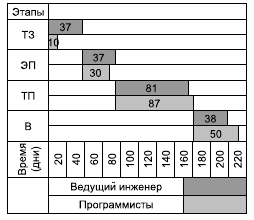
\includegraphics{econ_1.png}
	\caption{Календарный ленточный план работ.}
	\label{pic:econ_1}
\end{figure}

\begin{table}
    \centering
	\begin{tabularx}{\textwidth}{|c||X|X|X||X|X|X||X|X|X||X|X|X||c|}
		\hline
		& \multicolumn{3}{c||}{Г.И.} & \multicolumn{3}{c||}{П1} &
		\multicolumn{3}{c||}{П2} & \multicolumn{3}{c||}{П3..14} & Всего\\
		\hline
		Месяц & Р.Д. & ЗП & ЕСН & Р.Д. & ЗП & ЕСН & Р.Д & ЗП & ЕСН &
		Р.Д. & ЗП & ЕСН & за период\\
		\hline
		1 & 21 & 20 & 6 & 10 & 9.52 & 2.85 & & & & & & & 38.38\\
		\hline
		2 & 21 & 20 & 6 & 5 & 4.76 & 1.42 & & & & & & & 32.19\\
		\hline
		3 & 21 & 20 & 6 & 21 & 20 & 6 & & & & & & & 52\\
		\hline
		4 & 21 & 20 & 6 & 14 & 13.33 & 4 & 7 & 6.66 & 2 & 7 & 6.66 & 2 & 60.67\\
		\hline
		5 & 21 & 20 & 6 & 21 & 20 & 6 & 21 & 20 & 6 & 21 & 20 & 6 & 104.00\\
		\hline
		6 & 21 & 20 & 6 & 21 & 20 & 6 & 21 & 20 & 6 & 21 & 20 & 6 & 104.00\\
		\hline
		7 & 21 & 20 & 6 & 21 & 20 & 6 & 21 & 20 & 6 & 21 & 20 & 6 & 104.00\\
		\hline
		8 & 15 & 14.28 & 4.28 & 21 & 20 & 6 & 21 & 20 & 6 & 14 & 13.33 & 4 & 87.90\\
		\hline
		9 & 21 & 20 & 6 & 21 & 20 & 6 & 21 & 20 & 6 & & & & 78.00\\
		\hline
		10 & 10 & 9.52 & 2.85 & 22 & 20.95 & 6.28 & 22 & 20.95 & 6.28 & & & & 66.86\\
		\hline
		\multicolumn{13}{|l||}{Итого: } & 728.00 \\
		\hline
	\end{tabularx}
	\captionsetup{justification=centering}
	\caption{Затраты на зарплату и отчисления на социальное страхование, тыс.руб.}
	\label{table:econ_5}
\end{table}

\begin{table}[ht]
    \centering
	\begin{tabu}[\textwidth]{|X[c]|X[c]|X[c]|X[c]|X[c]|}
	\hline
	Наименование материала & Единица измерения & К-во & Цена/ед. (руб.) & Сумма (руб.) \\
	\hline
	Персональный компьютер & ASUS K52-JT & 14 & 25000 & 350000 \\
	\hline
	Офисная мебель & стулья и столы ikea & 14 & 5000 & 70000 \\
	\hline
	Бумага А4 & Пачка 500 листов & 2 & 200 & 400 \\
	\hline
	Картридж принтера Canon IP5200 & Картридж, 10мл & 5 & 300 & 1500 \\
	\hline
	\multicolumn{4}{|l|}{Итого:} & 421900 \\
	\hline
	\end{tabu}
	\captionsetup{justification=centering}
	\caption{Затраты на материалы.}
	\label{table:econ_6}
\end{table}

\subsubsection{Расчёт стоимости программного продукта}

Цена ПП рассчитывается по формуле:
$$Ц = С + Пр$$
$$Пр = \frac{(C - C_{M}) \cdot p_{Н}}{100\%}$$
где
\begin{itemize}
	\item $С$ - затраты на разработку ПП
	\item $С{м}$ - материальные затраты, руб./изд
	\item $Пр$ - желаемая прибыль
	\item $р_{н}$ - норматив рентабельности, принимаемый разработчиком
\end{itemize}

Тогда примем $Ц = 5 000 руб.$

Нужно продать 350 лицензионные копии, чтобы окупить вложенные средства.

\subsection{Рассчет экономической эффективности}

Основными показателями экономической эффективности является чистый
дисконтированный доход (ЧДД) и срок окупаемости вложенных средств.

Чистый дисконтированный доход определяется по формуле:
$$ЧДД = \sum^{T}_{t=0}(R_{t} - З_{t}) \frac{1}{(1 + E)^t}$$
где
\begin{itemize}
	\item $T$ - горизонт расчета по месяцам;
	\item $t$ - период расчета;
	\item $R_{t}$ - доход за текущий месяц;
	\item $З_{t}$ затраты за текущий месяц;
	\item $E$ - приемлемая для инвестора норма прибыли на вложенный капитал.
\end{itemize}

Коэффициент E установим равным ставке рефинансирования ЦБ РФ --
8.25\% годовых (или 0, 66\% в месяц). В виду особенности разрабатываемого
продукта он может быть продан лишь однократно. Коэффициент дисконти-
рования равен 1/(1 + Е) = 0,993.

В таблице~\ref{table:econ_6} приведен расчет ЧДД по месяцам работы над проектом.
График ЧДД приведён на рис.~\ref{pic:econ_2}.

\begin{table}
    \centering
	\begin{tabu}[\textwidth]{|c|c|c|c|c|}
	\hline
	Месяц & Тек. Затр. & Общ. Затр. & Тек.доход & ЧДД \\
	\hline
	1 & 46130,95 & 46130,95 & 0,00 & -45817,25 \\
	\hline
	2 & 39940,48 & 86071,43 & 0,00 & -85216,39 \\
	\hline
	3 & 59750,00 & 145821,43 & 0,00 & -143755,76\\
	\hline
	4 & 68416,67 & 214238,10 & 0,00 & -210330,39\\
	\hline
	5 & 111750,00 & 325988,10 & 0,00 & -318332,22\\
	\hline
	6 & 111750,00 & 437738,10 & 0,00 & -425599,63\\
	\hline
	7 & 111750,00 & 549488,10 & 0,00 & -532137,62\\
	\hline
	8 & 95654,76 & 645142,86 & 0,00 & -622710,94\\
	\hline
	9 & 85750,00 & 730892,86 & 0,00 & -703353,54\\
	\hline
	10 & 74607,14 & 805500,00 & 987500,00 & 149328,11 \\
	\hline
	\end{tabu}
	\captionsetup{justification=centering}
	\caption{Расчёт ЧДД (все значения в руб.).}
	\label{table:econ_6}
\end{table}

\begin{figure}
    \centering
	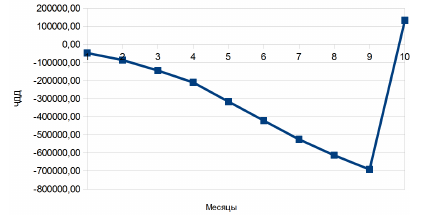
\includegraphics{econ_2.png}
	\caption{График изменения чистого дисконтированного дохода.}
	\label{pic:econ_2}
\end{figure}

\subsection*{Выводы}
\addcontentsline{toc}{subsection}{Выводы}

Согласно проведённым расчётам, проект является рентабельным. Итоговый
ЧДД составил $149328.11$ рублей. Срок реализации проекта равен 10 месяцам.

Поскольку программный продукт - рентабелен, он окупится после выхода на рынок.
Учитывая курс правительства РФ на модернизацию науки и техники, следует
ожидать повышенный спрос не только на конкретную реализацию, а также на
научный труд, подкрепляющий данную реализацию. Также данный программный
продукт может быть использован в широком спектре ниш: распознавание в метро,
при входе на предприятие, автоматическая блокировка ПК, домашние двери.
Это позволяет предположить, что программный продукт не только окупится,
но и принесет ощутимую прибыль при его должном развитии.
\clearpage

	\newpage
    \section{Условия труда}
В настоящем разделе будут рассмотрены условия, в которых
находился работник при разработке программного обеспечения.

\subsection{Анализ опасных и вредных факторов при разработке программного
    обеспечения и мероприятия по их устранению}

Разработка программного обеспечения требует постоянного взаимодействия с
вычислительными машинами, что связано с воздействием ряда вредных и зачастую опасных факторов, таких
как статическое электричество, рентгеновское излучение, электромагнитные поля,
ультрафиолетовое излучение, блики, отраженный свет и мерцание изображения.
Рассмотрим более подробно некоторые из вышеуказанных факторов.

\subsubsection{Микроклимат}

Работа за компьютером не требует серьезных физических усилий, поэтому ее относят к категории \textit{1а}.
Оптимальные нормы микроклимата для этой категории определяются таблицей \textit{СанПиН 2.2.2/2.4.1340-03}
(таблица~\ref{tables:microclimate}).

\begin{table}[hbt!]
\centering
\begin{tabu}[\textwidth]{|X[c]|X[c]|X[c]|X[c]|}
    \hline
    & Температура воздуха,~\celsius & Относительная влажность воздуха,~\% & Скорость движения воздуха, $ м/с $ \\
    \hline
    Холодный & 22-24 & 40-60 & 0.1 \\
    \hline
    Теплый & 23-25 & 40-60 & 0.1 \\
    \hline
\end{tabu}
\caption{Оптимальные нормы микроклимата}
\label{tables:microclimate}
\end{table}

Вредным фактором при работе с ЭВМ является также запыленность помещения. Этот фактор усугубляется влиянием на частицы пыли
электростатических полей персональных компьютеров.

Для устранения несоответствия параметров указанным нормам проектом предусмотрено использование системы кондиционирования как
наиболее эффективного и автоматически функционирующего средства.

Нормы \textit{СанПиН 2.2.4.1294-03} <<Санитарно-гигиенические нормы допустимых уровней ионизации воздуха>> определяют уровни положительных и
отрицательных ионов в воздухе (таблица~\ref{tables:gigenic}):

\begin{table}[hbt!]
\centering
\begin{tabu}[\textwidth]{|X[c]|X[c]|X[c]|}
    \hline
    \multirow{2}{*}{Уровни} & \multicolumn{2}{c|}{Число ионов в 1 см куб. воздуха} \\
    \cline{2-3}
    & $ n^+ $ & $ n^- $ \\
    \hline
    Минимально необходимые & 400 & 600 \\
    \hline
    Оптимальные & 1500-3000 & 3000-5000 \\
    \hline
    Предельно допустимые & 50000 & 50000 \\
    \hline
\end{tabu}
\caption{Уровни ионизации воздуха помещений при работе на ВДТ и ПЭВМ}
\label{tables:gigenic}
\end{table}

Для обеспечения требуемых уровней предусмотрено использование системы ионизации \textit{Сапфир-4А}.

Концентрация вредных химических веществ в помещениях с ПЭВМ не должна превышать <<ПДК загрязняющих веществ в атмосферном воздухе
населенных мест>> \textit{ГН 2.1.6.789-99}. Для выполнения указанных требований предусмотрено применение фильтров из активированного угля.

\subsubsection{Шум и вибрации}

Уровень шума на рабочем месте программиста не должен превышать 50 дБА, а уровень вибрации не должен превышать допустимых норм
вибрации. \textit{СанПиН 2.2.2.542-96} устанавливает следующие нормы на вибрацию (таблица \ref{tables:vibration}).
\begin{table}[hbt!]
\centering
\begin{tabu}[0.8\textwidth]{|X[c]|X[c]|X[c]|}
    \hline
    Среднегеометрические & \multicolumn{2}{c|}{Допустимые значения} \\
    частоты октавных полос, Гц & \multicolumn{2}{c|}{по виброскорости} \\
    \cline{2-3}
    & $ \times 10, м/с $ & $ дБ $ \\
    \hline
    2 & 4.5 & 79 \\
    \hline
    4 & 2.2 & 73 \\
    \hline
    8 & 1.1 & 67 \\
    \hline
    16 & 1.1 & 67 \\
    \hline
    31.5 & 1.1 & 67 \\
    \hline
    63 & 1.1 & 67 \\
    \hline
    Корректированные значения и их уровни & 2.0 & 72 \\
    \hline

\end{tabu}
\caption{Допустимые нормы вибрации на рабочих местах с ВДТ и ПЭВМ}
\label{tables:vibration}
\end{table}

При разработке программного обеспечения внутренними источниками шума являются вентиляторы, а также принтеры и другие периферийные
устройства ЭВМ. 

Внешние источники шума -- прежде всего, шум с улицы и из соседних помещений. Постоянные внешние источники шума, превышающего нормы,
отсутствуют.

Для устранения превышения нормы проектом предусмотрено применение звукопоглощающих материалов для облицовки стен и потолка
помещения, в котором осуществляется работа с вычислительной техникой.


\subsubsection{Освещение}
Наиболее важным условием эффективной работы программистов и пользователей является соблюдение оптимальных параметров системы
освещения в рабочих помещениях.

Естественное освещение осуществляется через светопроемы, ориентированные в основном на север и северо-восток (для исключения
        попадания прямых солнечных лучей на экраны компьютеров) и обеспечивает коэффициент естественной освещенности (КЕО) не ниже
1,5\%.

В качестве искусственного освещения проектом предусмотрено использование системы общего равномерного освещения. В соответствии с
\textit{СанПиН 2.2.2/2.4.1340-03},  освещенность на поверхности рабочего стола находится в пределах 300-500 лк. Разрешается использование
светильников местного освещения для работы с документами (при этом светильники не должны создавать блики на поверхности экрана).

Правильное расположение рабочих мест относительно источников освещения, отсутствие зеркальных поверхностей и использование матовых
материалов ограничивает прямую (от источников освещения) и отраженную (от рабочих поверхностей) блескость. При этом яркость
светящихся поверхностей не превышает 200 кд/кв.м, яркость бликов на экране ПЭВМ не превышает 40 кд/кв.м, и яркость потолка не
превышает 200 кд/кв.м.

В соответствии с \textit{СанПиН 2.2.2/2.4.1340-03}  проектом предусмотрено использование люминесцентных ламп типа ЛБ в качестве источников
света при искусственном освещении. В светильниках местного освещения допускается применение ламп накаливания.

Применение газоразрядных ламп в светильниках общего и местного освещения обеспечивает коэффициент пульсации не более 5\%.
Таким образом, проектом обеспечиваются оптимальные условия освещения рабочего помещения.

\subsubsection{Рентгеновское излучение}
В соответствии с \textit{СанПиН 2.2.2/2.4.1340-03}, проектом предусмотрено использование ПЭВМ, конструкция которых обеспечивает мощность
экспозиционной дозы рентгеновского излучения в любой точке на расстоянии 0,05 м. от экрана и корпуса монитора не более 0,1
мбэр/час (100 мкР/час). Результаты сравнения норм излучения приведены в таблице \ref{tables:rentgen}.

\begin{table}[hbt!]
\centering
\begin{tabu}[\textwidth]{|X[c]|X[c]|}
    \hline
    & Допустимое значение, $ мкР/час $, не более \\
    \hline
    СанПиН 2.2.2/2.4.1340-03 & 100 \\
    \hline
    TCO-99 & 500 \\
    \hline
    MPR II & 500 \\
    \hline
\end{tabu}
\caption{Сравнение норм рентгеновского излучения в различных стандартах}
\label{tables:rentgen}
\end{table}

Как видно из таблицы \ref{tables:rentgen}, стандарты \textit{MPR II} и \textit{TCO-99} предъявляют менее жесткие требования к
рентгеновскому излучению, чем СанПиН. Но
при соблюдении оптимального расстояния между пользователем и монитором дозы рентгеновского излучения не опасны для большинства
людей.

\subsubsection{Неионизирующие электромагнитные излучения}

В соответствии с \textit{санпин 2.2.2/2.4.1340-03}, допустимые значения параметров неионизирующих излучений приводятся в таблицах
    \ref{tables:electric} и \ref{tables:magnet}.
\begin{table}[hbt]
\centering
\begin{tabu}[\textwidth]{|X[c]|X[c]|}
    \hline
    Диапазон частот, $ \times 10^3 $, гц & Допустимые значения, $В/м$ \\
    \hline
    $ 5 \times 10^{-3}$ --- 2 & 25 \\
    \hline
    2 --- 400 & 2.5 \\
    \hline
\end{tabu}
\caption{Предельно допустимые значения напряженности электрического поля}
\label{tables:electric}
\end{table}

\begin{table}[hbt]
\centering
\begin{tabu}[\textwidth]{|X[c]|X[c]|}
    \hline
    Диапазон частот, $ \times 10^3 $, гц & Допустимые значения, $нТл$ \\
    \hline
    $ 5 \times 10^{-3}$ --- 2 & 250 \\
    \hline
    2 --- 400 & 25 \\
    \hline
\end{tabu}
\caption{Предельно допустимые значения плотности магнитного потока}
\label{tables:magnet}
\end{table}

Величина поверхностного электростатического потенциала не должна превышать 500 В. 

Мониторы, используемые в настоящее время, удовлетворяют нормам \textit{MPR II} (или более жестким требованиям) и имеют предельные
значения, указанные в таблицах \ref{tables:electromagnet} и \ref{tables:induction}
\begin{table}[hbt]
\centering
\begin{tabu}[\textwidth]{|X[c]|X[c]|}
    \hline
    Диапазон частот, $ \times 10^3 $, гц & Допустимые значения, $В/м$ \\
    \hline
    $ 5 \times 10^{-3}$ --- 2 & 25 \\
    \hline
    2 --- 400 & 2.5 \\
    \hline
\end{tabu}
\caption{Предельно допустимые значения напряженности электромагнитного поля}
\label{tables:electromagnet}
\end{table}

\begin{table}[hbt]
\centering
\begin{tabu}[\textwidth]{|X[c]|X[c]|}
    \hline
    Диапазон частот, $ \times 10^3 $, гц & Допустимые значения, $нТл$ \\
    \hline
    $ 5 \times 10^{-3}$ --- 2 & 200 \\
    \hline
    2 --- 400 & 25 \\
    \hline
\end{tabu}
\caption{Предельно допустимые значения магнитной индукции}
\label{tables:induction}
\end{table}

Поверхностный электростатический потенциал не превышает 500 В.

Таким образом, параметры электрических и магнитных (неионизирующих) полей удовлетворяют требованиям \textit{СанПиН}.

\subsubsection{Визуальные параметры}

Неправильный выбор визуальных эргономических параметров приводит к ухудшению здоровья пользователей, быстрой утомляемости,
раздражительности. В этой связи, проектом предусмотрено, что конструкция вычислительной системы и ее эргономические параметры
обеспечивают комфортное и надежное считывание информации.

Требования к визуальным параметрам, их внешнему виду, дизайну, возможности настройки представлены в \textit{СанПиН 2.2.2/2.4.1340-03}.
Визуальные эргономические параметры монитора и пределы их изменений приведены в таблице \ref{tables:vdt_params}.
\begin{table}[hbt]
\centering
\begin{tabu}[\textwidth]{|X[c]|X[c]|X[c]|}
    \hline
    Наименование & \multicolumn{2}{c|}{Пределы значений параметров} \\
    \cline{2-3}
    параметров & минимальные (не менее) & максимальные (не более) \\
    \hline
    Яркость знака (яркость фона), $ кд/кв.м. $ (измеренная в темноте) & 35 & 120 \\
    \hline
    Внешняя освещенность экрана, $ лк $ & 100 & 250 \\
    \hline
    Угловой размер знака, $ угл.мин. $ & 16 & 60 \\
    \hline
\end{tabu}
\caption{Допустимые нормы вибрации на рабочих местах с ВДТ и ПЭВМ}
\label{tables:vdt_params}
\end{table}

Для выполнения этих требований проектом предусмотрено использование современных мониторов, имеющих достаточно широкий набор
регулируемых параметров. В частности, для удобного считывания информации реализована возможность настройки положения монитора по
горизонтали и вертикали. Мониторы оснащены специальными устройствами и средствами настройки ширины, высоты, яркости, контраста и
разрешения изображения. Кроме того, в современных мониторах зерно изображения имеет размер в пределах 0,27 мм, что обеспечивает
высокую четкость и непрерывность изображения. Наконец, на поверхность дисплея нанесено матовое покрытие, чтобы избавиться от
солнечных бликов.

\subsection{Расчет уровней звукового давления в помещении}

На рисунке \ref{pic:noises} изображена схема расположения расчетной точки относительно источников шума, при этом,
источники шума 1 и 3 находится на полу, а источник 2 находится в подвешенном состоянии.

\begin{figure}[tbh]
\centering
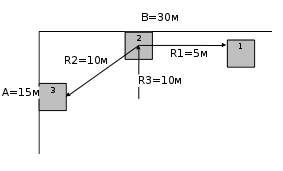
\includegraphics[width=0.6\textwidth]{noise}
\caption{Схема расположения расчетной точки относительно источников шума}
\label{pic:noises}
\end{figure}

Уровни звуковой мощности источников ($ L_p = f(f_{cr}) $) представлены в таблице~\ref{table:noise_lvl}.
Габаритные размеры помещения, $ A \times B \times C, м^3 $, $15 \times 30 \times 4$.
\begin{table}[bth]
\centering
    \begin{tabu}{|X[3,c]|X[1,c]|X[1,c]|X[1,c]|}
        \hline
        & Источник 1 & Источник 2 & Источник 3 \\
        \hline
        Уровень звуковой мощности & 9 & 1 & 8 \\
        \hline
    \end{tabu}
    \caption{Уровни звуковой мощности источников}
    \label{table:noise_lvl}
\end{table}

Объем помещения:
$$ V = A \cdot B \cdot C = 15 \cdot 30 \cdot 4 = 1800\ м^3 $$
Использумые обозначения:
\begin{itemize}
    \item $ \mu $ -- частотный множитель;
    \item $ \Phi = 1 $ -- фактор направленности источника шума;
    \item $ \chi = 1 $ -- коэффициент влияния ближнего акустического поля;
    \item $ y = 1 $ -- диффузность звукового поля в помещении.
\end{itemize}

Уровни интенсивности звука расчитываются по формуле:
$$ L_j = L_p + 10 \lg{(\frac{\Phi\chi}{S} + \frac{4y}{B})} $$

В таблице \ref{table:noise} представлены расчеты уровня звукового давления, а в таблице \ref{table:noise_intence}
представлены расчеты уровня звуковой интенсивности.

\begin{table}[bth]
\centering
    \begin{tabu}[\textwidth]{|X[5,c]|X[1,c]|X[1,c]|X[1,c]|X[1,c]|X[1,c]|X[1,c]|X[1,c]|X[1,c]|X[2,c]|}
        \hline
        Источник & \multicolumn{8}{c|}{Уровни звуковой мощности} & S \\
        \cline{2-9}
        & 63 & 125 & 250 & 500 & 1000 & 2000 & 4000 & 8000 & \\
        \hline
        \textnumero1, на полу, 5м & 90 & 91 & 98 & 99 & 97 & 93 & 91 & 86 & 157 \\
        \hline
        \textnumero2, подвешен, 10м & 84 & 82 & 84 & 91 & 94 & 94 & 91 & 91 & 314 \\
        \hline
        \textnumero3, на полу, 10м & 101 & 102 & 100 & 101 & 99 & 99 & 97 & 91 & 314 \\
        \hline
    \end{tabu}
    \caption{Параметры расчетов уровня звукового давления}
    \label{table:noise}
\end{table}

\begin{table}[bth]
\centering
    \begin{tabu}[\textwidth]{|X[3,c]|X[1,c]|X[1,c]|X[1,c]|X[1,c]|X[1,c]|X[1,c]|X[1,c]|X[1,c]|}
        \hline
        & \multicolumn{8}{c|}{Уровни звуковой интенсивности} \\
        \cline{2-9}
        & 63 & 125 & 250 & 500 & 1000 & 2000 & 4000 & 8000 \\
        \hline
        $Y$ & 0.8 & 0.75 & 0.7 & 0.8 & 1 & 1.4 & 1.8 & 2.5 \\
        \hline
        $B$ & 72 & 67.5 & 63 & 72 & 90 & 126 & 162 & 225 \\
        \hline
        Источник \textnumero1 & $ 77.919 $ & $ 79.171 $ & $ 86.442 $ & $ 86.919 $ & $ 84.060 $ & $ 78.811 $ & $ 75.922 $ & $ 69.829 $ \\
        \hline
        Источник \textnumero2 & $ 71.689 $ & $ 69.955 $ & $ 72.240 $ & $ 78.689 $ & $ 80.779 $ & $ 79.432 $ & $ 75.452 $ & $ 74.214 $ \\
        \hline
        Источник \textnumero3 & $ 88.689 $ & $ 89.955 $ & $ 88.240 $ & $ 88.689 $ & $ 85.779 $ & $ 84.432 $ & $ 81.452 $ & $ 74.214 $ \\
        \hline
        $ L_{max} $ & 83 & 74 & 68 & 63 & 60 & 57 & 55 & 54 \\
        \hline
        $ L_{j_{sum}} $ & 89.118 & 90.343 & 90.509 & 91.157 & 88.766 & 86.447 & 83.302 & 77.951 \\
        \hline
    \end{tabu}
    \caption{Параметры расчетов уровня звуковой интенсивности}
    \label{table:noise_intence}
\end{table}

Суммарный шум рассчитывается по следующей формуле:
$$ L_{j_{sum}} = 10\lg{(\sum_{i} 10^{\frac{L_i}{10}})} $$

\begin{figure}[bth]
\centering
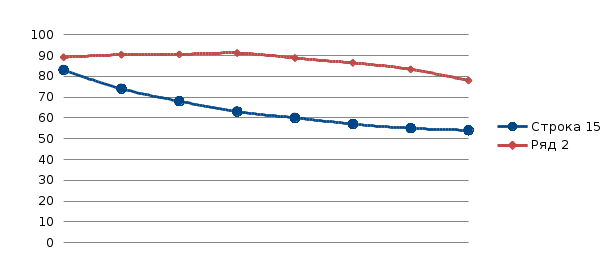
\includegraphics[width=0.8\textwidth]{noise_graph}
\caption{График распределения расчетного спектра уровня шума относительно предельно допустимых значений}
\label{pic:noise_graph}
\end{figure}

\subsubsection*{Выводы}
На рисунке \ref{pic:noise_graph} видно, что расчетный спектр превышает предельно допустимый уровень шума, причем на всех октавных частотах.
Замечено, что увеличение расстояния до источников шума довольно слабо влияет на его уровень.
Если изменить габариты помещения, то это может значительно повлиять на уровень шума в данном помещении в целом,
однако все равно не позволяет снизить его до допустимых значений. Рекомендованным защитным мероприятием в данном
случае будет являться акустическая обработка помещения, а также применение звукоизоляции.

\subsection{Расчет системы искусственного освещения}

С помощью программы DIALux были произведены расчеты, результаты которых представлены на рисунках \ref{pic:light_1},
\ref{pic:light_2}, \ref{pic:light_3}, \ref{pic:light_4} и \ref{pic:light_5}, при этом использовались
следующие параметры:
\begin{itemize}
    \item Габариты помещения: $ 7 \times 4 \times 2.8 $ (м);
    \item Коэффициенты отражения:
        \begin{itemize}
            \item Потолок: 31\% (медово-желтый цвет);
            \item Стены: 28\% (бежевый цвет);
            \item Пол: 18\% (Красно-оранжевый цвет);
        \end{itemize}
    \item Высота рабочей плоскости: 0.85 м;
    \item Планируемая освещенность: $ E = 300 лк. $
\end{itemize}

\begin{figure}[p]
\centering
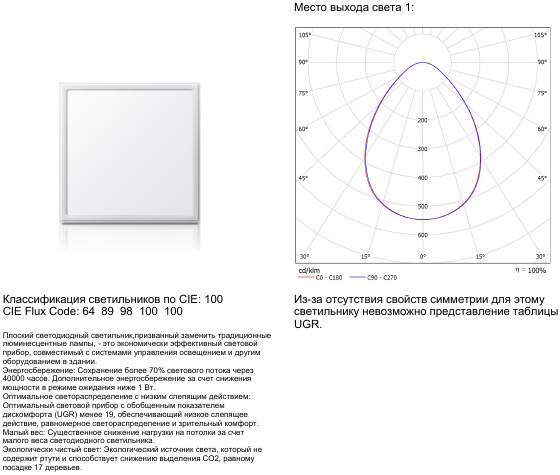
\includegraphics[width=\textwidth]{lights_1}
\caption{Паспорт светильника}
\label{pic:light_1}
\end{figure}
\begin{figure}[p]
\centering
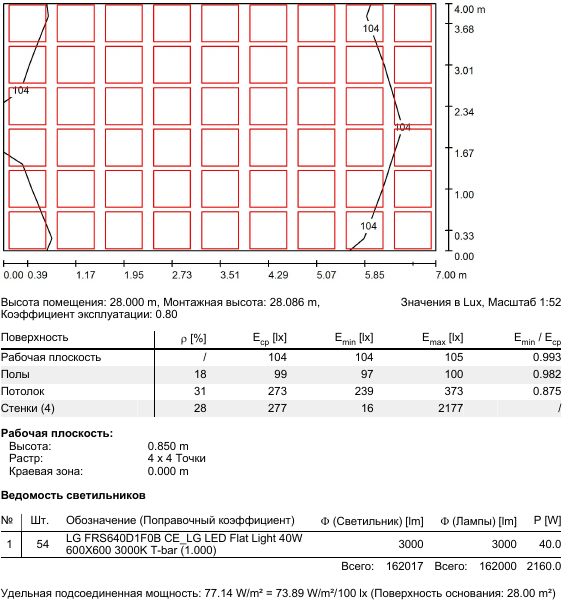
\includegraphics[width=\textwidth]{lights_2}
\caption{Резюме помещения}
\label{pic:light_2}
\end{figure}
\begin{figure}[p]
\centering
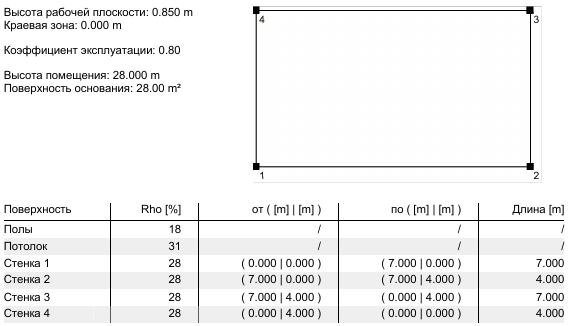
\includegraphics[width=\textwidth]{lights_3}
\caption{Протокол ввода помещения}
\label{pic:light_3}
\end{figure}
\begin{figure}[p]
\centering
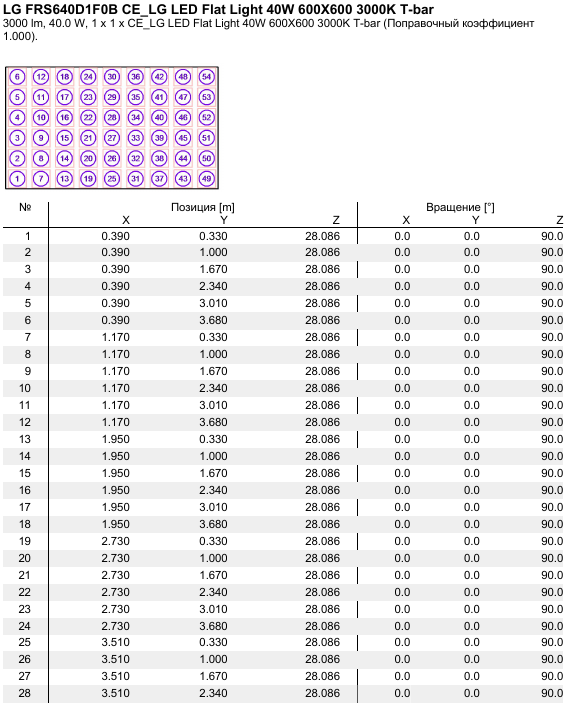
\includegraphics[width=\textwidth]{lights_4}
\caption{Светильники}
\label{pic:light_4}
\end{figure}
\begin{figure}[p]
\centering
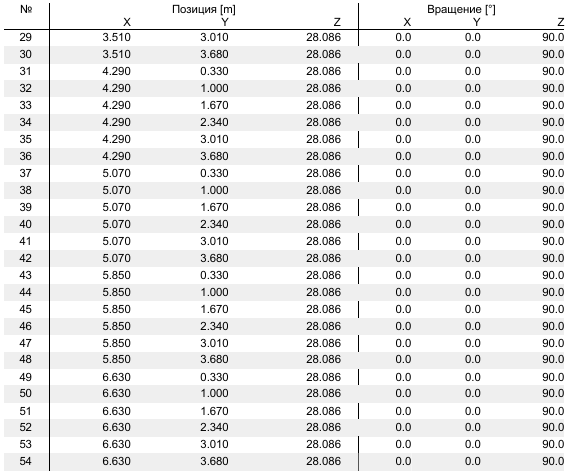
\includegraphics[width=\textwidth]{lights_5}
\caption{Светильники, список координат}
\label{pic:light_5}
\end{figure}
\FloatBarrier

\subsection*{Выводы}
\addcontentsline{toc}{subsection}{Выводы}

Согласно проведенным расчетам, условия, в которых происходила разработка программного продукта,
являются приемлимыми и не оказывают серьезного негативного воздействия на работника.
\clearpage

%	\section{Введение}

Автоматический анализ лиц, который включает в себя обнаружение лиц,
распознавание лиц, распознавание эмоций на лицах, в настоящее время является активно развивающейся областью машинного зрения. Коммерческие,
охранные и другие анализирующие приложения все чаще используют технологию распознавания лиц для сбора информации. Лицо человека является
одним из его главных идентификаторов. Очевидно, что лицо - наиболее видимая часть человеческого тела в обыденной жизни. По нему можно
определить личность человека, а также попробовать определить его эмоциональный настрой.

Каждый из нас имеет уникальные черты лица, которые являются одной из достоверных отличительных особенностей. Распознавание
лиц производится с целью сопоставления лица на входном изображению кластеру изображений лиц в базе данных с некоей точностью. Данный кластер
может состоять как из изображения одного лица, так и из нескольких изображений, принадлежащих одному человеку, что в свою очередь увеличивает
точность распознавания. Актуальность проблемы подтверждает заинтересованность в ней такого технологического гиганта, как Facebook. Например,
согласно \cite{facebook} им удалось вплотную приблизиться к точности распознавания,
сравнимой с человеческой.

С ростом популярности мобильных устройств, увеличивается необходимость в повышении безопасности при доступе к мобильному устройству.
Одним из методов идентификации личности пользователя устройства, является идентификация по внешним признакам.

Целью работы является улучшение показателей распознавания лиц в реальном времени и практическое применение
разработанных алгоритмов в мобильном устройстве.
Среди таких показателей можно выделить скорость работы программы, точность распознавания и количество оперативной памяти,
требуемой при распознавании.

Для достижения поставленной цели необходимо рассмотреть из каких
этапов состоит распознавание лиц и улучшить те этапы, которые сильнее
всего влияют на вышеуказанные показатели. Согласно \cite{facebook} распознавание лиц
состоит из: обнаружения, выравнивания, представления информации о лице
в виде, пригодной для распознавания и, собственно, распознавания. Данная
работа посвящена решению задачи поиска лица на фотоснимке, представлению информации о лице
и последующей классификации.

Методы обнаружения лица должны давать как можно более однозначные результаты, имея при этом
минимальную погрешность. Также важными являются факторы скорости работы,
затрат оперативной памяти и возможность распараллеливания. Алгоритмы обнаружения и
классификации должны работать в реальном времени с низким числом ложных срабатываний.

В аналитическом разделе выполняется обзор предметной области. Рассматриваются существующие методы решения проблем, сравниваются
результаты их работы. Обосновывается выбор настоящего решения. В конструкторском разделе описываются используемые методы или алгоритмы.
Также в нем описываются выбранные способы тестирования, результаты тестирования и структура разрабатываемого программного обеспечения.
Технологический раздел содержит обоснованный выбор средств программной
реализации, описание основных моментов программной реализации и методики
тестирования созданного программного обеспечения. В нем же описывается информация,
необходимая для сборки и запуска разработанного программного обеспечения. В экспериментальном разделе содержится описание
планирования экспериментов и их результаты.

\clearpage
	
%	\input{analizis}
%	\subsection{Конструкторский раздел}

Lalala

\subsection{Метод Виолы-Джонса}

Хотя метод был разработан и представен еще в 2001 году Полом Виолой и Майклом
Джонсом \cite{viola_jones}, он до сих пор является основополагающим для поиска
объектов на изображении в реальном времени.
Алгоритм может распознавать различные классы изображений, однако основной задачей
при его создании было обнаружение лиц.

Существует множество реализаций этого метода, в том числе в составе библиотеки
компьютерного зрения OpenCV \cite{opencv}.

Основные принципы, на которых реализован алгоритм, таковы:
\begin{itemize}
    \item используются изображения в интегральном представлении,
        что позволяет вычислять быстро необходимые объекты;
    \item используются признаки Хаара, с помощью которых происходит
        поиск нужного объекта (в данном контексте, лица и его черт);
    \item используется бустинг (от англ. \textit{boost}~-- улучшение,
        усиление) для выбора наиболее подходящих признаков для искомого
        объекта на данной части изображения;
    \item все признаки поступают на вход классификатора,
        который даёт результат <<верно>> либо <<ложь>>;
    \item используются каскады признаков для быстрого отбрасывания окон,
        где не найдено лицо.
\end{itemize}

Обучение классификаторов идет очень медленно, но результаты поиска
лица очень быстры, именно поэтому был выбран данный метод
распознавания лиц на изображении. Виола-Джонс является
одним из лучших по соотношению показателей эффективность
распознавания/скорость работы. Также этот детектор
обладает крайне низкой вероятностью ложного обнаружения лица. Алгоритм
даже хорошо работает и распознает черты
лица под небольшим углом, примерно до 30 градусов. При угле
наклона больше 30 градусов
процент обнаружений резко падает.

Данный метод в общем виде ищет лица и черты лица по общему
принципу сканирующего окна.

\clearpage

%	\section{Технологический раздел}

В данном разделе будут рассмотрены 
средства программной 
реализации, описание основных моментов программной реализации и 
методики тестирования созданного программного обеспечения. 

\subsection{Технические средства}

В данном разделе будут описаны технические средства, которые
были использованы в процессе разработки программного обеспечения.

\subsubsection{Язык программирования}

Для разработки был выбран язык программирования C++. Из его достоинств следует
выделить высокую скорость (практически сравнимую с языком C для современных
компиляторов) и широкие возможности, позволяющие достаточно писать достаточно
удобный и выразительный код по сравнению с тем же C, а так же вероятно самое
большое количество удобных сторонних библиотек на все случаи жизни. Также C++
предоставляет громоздкие, но крайне эффективные методы шаблонного
метапрограммирования, позволяющие генерировать очень эффективный код из
неповторяющихся блоков. Из недостатков следует выделить относительную сложность синтаксиса и
большое количество правил языка и нетривиальных моментов в языке, из чего
следует потенциально большое количество скрытых ошибок.

Было выбрано подмножество языка C++11, которое даёт разработчику новые
возможности по написанию более быстрого и понятного кода, большие приятные
нововведения в библиотеку C++ STL, а так же новые конструкции для избавления от
некоторых ошибок.

В качестве альтернатив рассматривались некоторые , скриптовые языки общего назначения с
привязками к библиотекам с машинным кодом (Python, Ruby, Perl), языки общего
назначения со сборкой мусора, исполняемые на виртуальной машине (Java,
Scala). Поскольку проект предполагает громоздкие вычисления с необходимостью
расчётов в реальном времени, был сделан выбор в пользу компилируемых в машинный
код языков программирования, среди которых был выбран C++ как наиболее удобный и
функциональный, а также как один из самых быстрых.  На момент начала работы
основные аспекты языка уже были изучены, что позволило целиком
сконцентрироваться на задаче, а не тратить время на изучения инструмента.

\subsubsection{Компилятор}

В процессе разработки использовался компилятор языка C++ GCC.
Он представляет собой самый развитый и популярный свободный
компилятор для языка C++ в мире, включает в себя большое множество оптимизаций,
поддерживаемых платформ и генерирует крайне эффективный код.
Компилятор был выбран по соображениям
большого количества поддерживаемых платформ, в том числе Linux, на котором в
основном разрабатывался данный проект.

\subsubsection{Утилиты и среды разработки}

Проект разрабатывался в нескольких средах разработки. В основном разработка
делилась на два цикла~-- написание кода и отладка. Для написания кода
использовалась среда разработки QtCreator. Эта среда предоставляет
разработчику удобные средства создания кода, включая интуитивную подсветку синтаксиса
библиотеки Qt5 и встроенный отладчик.
Альтернативами приведённым инструментам является текстовый редактор
EMacs и интерфейс отладчика GDB CGDB, предоставляющий консольный
псевдo-оконный интерфейс для работы.

Написание пояснительной записки к проекту производилось в текстовом редакторе Vim с набором расширений, обеспечивающих
предельно комфортную работу с исходным кодом на языке \verb|C++| и \TeX.

\subsubsection{Поиск ошибок}

В процессе разработки использовался свободный кроссплатформенный отладчик GNU
GDB, предоставляющий широкие возможности по отслеживанию выполнения программы,
поиску ошибок и изучению её работы. Также в процессе разработки использовался
статический анализатор кода CppCheck, указывающий на множество незамеченных и
неочевидных ошибок в исходном коде на основе его анализа. Для поиска ошибок
выделения памяти использовался анализатор памяти Valgrind, результатом работы
которого является список потенциальных утечек памяти, использований
освобождённой памяти и других ошибок работы с ней. Для измерения скорости работы
частей программы и нахождения узких мест использовался комплекс для измерения
производительности Valgrind, предоставляющий табоицу функций программы со
множеством статистических и временных данных.

\subsubsection{Основная библиотека}

В качестве основной библиотеки разработки приложения использовалась библиотека с
открытым исходным Qt5,
которая позволяет разрабатывать кроссплатформенные приложения с одинаковым
программным функционалом. Библиотека в том числе позволяет разрабатывать приложения
для устройств под управлением ОС Android, на которую в основном нацелена данная работа.
Библиотека может свободно использоваться в проектах и в академических и в коммерческих целях.

Кроме того библиотека позволяет в автоматическом режиме формировать установочный пакет,
который будет использоваться при установке приложения на мобильное устройство.
Все необходимые зависимости, а так же обертки для классов языка \verb|C++| в язык Java
библиотека формирует так же сама.

При реализации нейронной сети была использована библиотека FANN\cite{fann}. FANN~--
нейросетевая библиотека с открытым исходным кодом, которая реализует многослойные искуственные
нейронные сети на языке С. Библиотека является кросс-платформенной, она проста в использовании
универсальна, хорошо документирована и быстра.

\subsubsection{Тестирование}

Для написания тестов был использован Google C++ Testing Framework, который
является библиотекой для модульного тестирования на языке \verb|C++|. Google
Test построена на методологии тестирования xUnit, то есть когда отдельные части
программы (классы, функции, модули) проверяются отдельно друг от друга, в
изоляции.

\subsubsection{Сборка и запуск разработанного программного обеспечения}

Проект собирался при помощи системы сборки проектов QMake. Она была выбрана
из-за большой гибкости, простоты подключения и линковки сторонних библиотек и
удобства и относительной простоты файлов описания процесса сборки.

Для сборки разработанного программного обеспечения необходимо склонировать
репозиторий с исходным кодом или скопировать папку с ним к себе на ПК. После этого
достаточно последовательно запустить утилиты qmake и make.

\subsubsection{Документация}

С помощью утилиты Doxygen были сгенерированы диаграммы, отображающие
взаимосвязи исходного кода. Это позволяет <<увидеть>> архитектуру,
не читая все исходные файлы проекта.

\subsubsection{Сопроводительные записки}

Техническое задание, расчётно-пояснительная записка и прочее верстались
в системе вёрстки \LaTeX. Это дало возможность сконцетрироваться на
тексте вместо его оформления, получая красивую вёрстку <<из коробки>>, множество
удобных средств для оформления текста и прочее.

\subsection{База данных}

В процессе работы программа использует СУБД SQLite~-- компактная
встраиваемая реляционная база данных с открытым кодом. SQLite является системой
управления базами данных по умолчанию в мобильных устройствах под управлением ОС Android.

Система является очень компактной, легковестной и кроссплатформенной.
Система имеет привязку к самым различным
языкам программирования, таким, как Delphi, \verb|C++|, Java, \verb|C#|, VB.NET, Python, Perl, PHP, PureBasic и другим.

СУДБ кроме того имеет набор ограничений, которые необходимо иметь в виду при разработке программного
обеспечения. Однако, на разработку данного проекта эти ограничения существенного влияния не оказали.

\subsubsection{Схема базы данных}

Схема базы данных может быть представлена ER-диаграммой, изображенной на рисунке \ref{fig:er_diagram}.

\begin{figure}[hbtp]
    \centering
    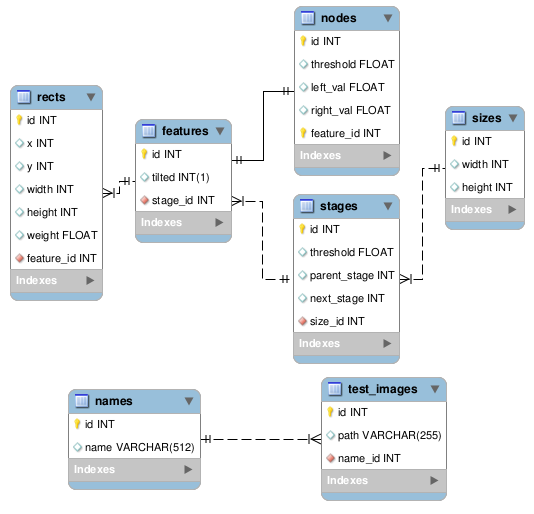
\includegraphics[width=\textwidth]{er_diagram.png}
    \caption{Схема базы данных}
    \label{fig:er_diagram}
\end{figure}

\subsubsection{Каскад Хаара}

В процессе работы приложения, алгоритм Виолы-Джонса использует стандартный каскад Хаара \cite{haar_cascade},
который был обучен ранее на большом объеме тестовых изображений.
Стандартный каскад представлен XML-документом и свободно доступен для загрузки.
Для более производительной работы приложения, каскад был перенесен из формата
XML в базу данных с помощью Perl-скрипта.

Приведем часть первого \textit{stage} из стандартного каскада:
\begin{verbatim}
<haarcascade_frontalface_alt>
  <size>20 20</size>
  <stages>
    <_>
      <!-- stage 0 -->
      <trees>
        <_>
          <!-- tree 0 -->
          <_> 
            <!-- root node -->
            <feature>
              <rects>
                <_>3 7 14 4 -1.</_>
                <_>3 9 14 2 2.</_></rects>
              <tilted>0</tilted></feature>
            <threshold>4.0141958743333817e-003</threshold>
            <left_val>0.0337941907346249</left_val>
            <right_val>0.8378106951713562</right_val></_></_>
        <_>
          <!-- tree 1 -->
          <_>
            <!-- root node -->
            <feature>
              <rects>
                <_>1 2 18 4 -1.</_>
                <_>7 2 6 4 3.</_></rects>
              <tilted>0</tilted></feature>
            <threshold>0.0151513395830989</threshold>
            <left_val>0.1514132022857666</left_val>
            <right_val>0.7488812208175659</right_val></_></_>
        ...
      # после всех признаков (деревьев) ...
      <stage_threshold>6.9566087722778320</stage_threshold>
      <parent>0</parent>
      <next>-1</next></_>
      ...
\end{verbatim}

Для хранения каскада Хаара в приложении были использованы следующие таблицы из
схемы, изображенной на рисунке \ref{fig:er_diagram}:

\begin{description}
    \item[rects] \hfill \\
        Таблица содержит массив прямоугольников, которые характеризуют
        конкретный признак. Так как каждый примитив Хаара представляет собой комбинацию из
        областей черного и белого цвета (рис. \ref{fig:haar}), при чем область черного цвета только одна,
        то для кодирования одного примитива достаточно следующих полей:
        \begin{description}
            \item[x] -- определяет горизонтальную координату темной части признака;
            \item[y] -- определяет вертикальную координату темной части признака;
            \item[width] -- определяет ширину темной части признака;
            \item[height] -- определяет высоту темной части признака.
        \end{description}
        Кроме того, при расчетах, используемых в алгоритме Виолы-Джонса используется
        вес каждого прямоугольного признака, который определен в поле \textbf{weight} таблицы.
        Каждый признак в каскаде Хаара может иметь более чем один примитив. Поэтому, в поле \textbf{feature\_id}
        для каждого примитива определено, к какому признаку он относится;
    \item[nodes] \hfill \\
        Таблица содержит список узлов каскада Хаара. Каждый узел характеризуется набором характеристик, среди
        которых выделяются:
        \begin{description}
            \item[threshold]~-- предельное значение, при преодолении которого узел можно считать отвергнутым;
            \item[left\_val]~-- значение, на которое будет увеличена характеристика признака в случае, если узел был отвергнут;
            \item[right\_val]~-- значение, на которое будет увеличена характеристика признака в случае, если узел был принят; 
            \item[feature\_id]~-- индекс признака, к которому относится данный узел.
        \end{description}
    \item[features] \hfill \\
        Таблица содержит список признаков, которыми оперирует алгоритм Виолы-Джонса.
        Каждый признак в общем случае может содержать только один узел, но при этом он содержит в себе
        множество примитивов. Каждый признак является частью одного этапа распознавания. При этом признаков в одном этапе
        может быть много. Идентификатор этапа хранится в поле \textbf{stage\_id}. Каждый признак кроме того может быть под
        наклоном. Этот факт кодируется в поле \textbf{tilted}. Так как в данном приложении используются только основные признаки
        Хаара, это поле всегда содержит 0. Однако, так как предполагается дальнейшая доработка программного продукта с
        добавлением дополнительных признаков, поле имеет место быть;
    \item[stages] \hfill \\
        Таблица содержит список этапов распознавания. Каждый этап состоит из набора признаков.
        В ходе алгоритма происходит накопление суммарных значений признаков на каждом этапе.
        В случае, если накопленное значение превысило значение \textbf{threshold}, этап отвергается и алгоритм
        переходит к следующему сканирующему окну. Для навигации по каскаду, используются поля
        \textbf{parent\_stage} и \textbf{next\_stage}. Кроме того, каждый этап ссылается на таблицу \textbf{sizes},
        определяя тем самым масштаб, который необходимо применить к сканируемому окну;
    \item[sizes] \hfill \\
        Таблица содержит список размеров примитивов. При этом в поле \textbf{width} определена ширина примитива, а в
        поле \textbf{height}~-- высота. Потенциально, алгоритм Виолы-Джонса способен работать с примитивами различного размера,
        повышая тем самым детализацию признаков. Однако, в текущей реализации программы используется лишь примитивы размера
        $20\times20$ точек и таблица была создана с целью увеличения функционала в будущем.
\end{description}

\subsubsection{Анализируемые объекты}

В ходе своей работы, программный продукт использует нейронную сеть для определения принадлежности анализируемого
изображения конкретной личности. Сами же личности должны быть сохранены в базе данных для последующего использования.

Именно эти данные хранит таблица \textbf{names}, при чем в поле \textbf{name} хранится полная информация о человеке.
Так как приложение не подразумевает, что для идентификации человека будет использовано именно его имя, то одного поля вполне
достаточно.

\subsubsection{Тестовые данные}

В ходе тестирования приложения был использован набор изображений из базы изображений под названием
\textit{Yale Face Database B} \cite{yale_face_database}. Она содержит более 16000 изображений 28ми человек в различных позах
и с различным углом наклона головы. Для хранения информации о местонахождении изображений на жестком диске
компьютера, на котором производится тестирование, используется таблица \textbf{test\_images}.

\subsection{Модульное тестирование}
Для разработанного программного обеспечения были написаны модульные тесты,
позволяющие проверить корректность ранее оттестированного кода при внесении
изменений. Пример прогонки модульных тестов показан на рисунке
\ref{fig:test}. Пример исходного кода модульных тестов представлен в приложенни
\ref{ap1}.

\begin{figure}[hbt]
  \centering
  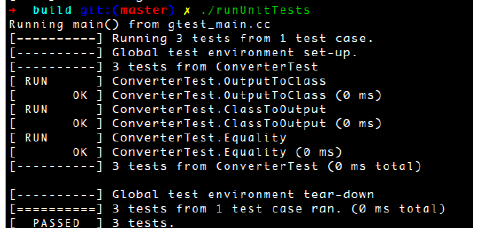
\includegraphics{tests.png}
  \caption{Пример прогона модульных тестов}
  \label{fig:test}
\end{figure}

\subsection{Структура программы}

Здесь мы опишем структуру программы, её основные элементы и устройство.
На рисунке \ref{fig:proj-struct} увидеть из каких модулей состоит программа.

\begin{figure}[h!]
  \centering
  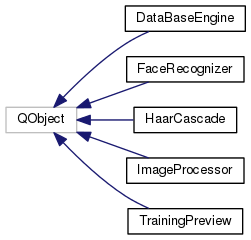
\includegraphics{uml.png}
  \caption{Структура программы}
  \label{fig:proj-struct}
\end{figure}

\subsection*{Выводы}
\addcontentsline{toc}{subsection}{Выводы}

Были рассмотрены основные методы, которые легли в основу разработанного
программного продукта. Была представлена и полностью описана схема базы данных,
была представлена диаграмма, показывающая структуру приложения.

\clearpage 
\section{Экспериментальный раздел}

В данном разделе будут представлены эксперименты, которые показывают
работоспособность созданного программного обеспечения.

\subsection{Достоверность распознавания}

Целью экспериментов является определение достоверности распознавания
разработанным программным продуктом. Достоверность распознавания определяется по
формуле
\[ \frac{TP}{TP+FP}, \]
где $TP$ - число правильно определенных объектов, $FP$ - число ложных обнаружений.


В эксперименте учавствуют 400 изображений, принадлежащие 40 людям.  Одно из
десяти изображений, принадлежащих одному человеку, является тестовым и не входит
в обучающую выборку.  В ходе экспериментов были получены результаты тестирования
скорости и достоверности распознавания. Результаты представлены на рисунке
\ref{fig:acc}.

\begin{figure}[h!]
  \centering
    \captionsetup{justification=centering}
  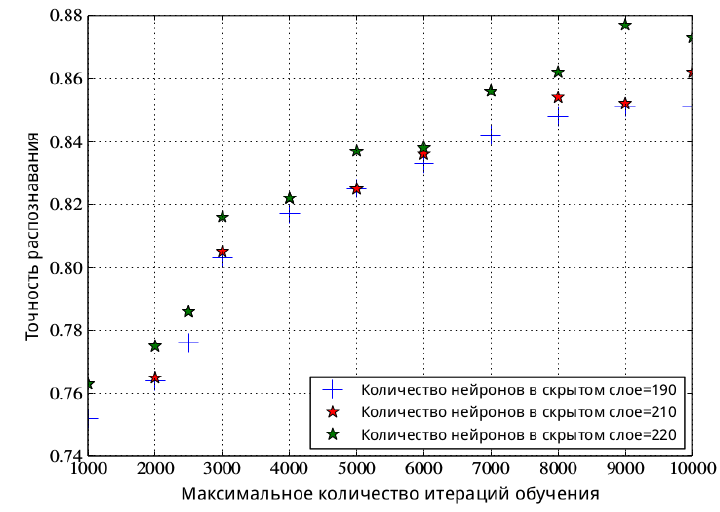
\includegraphics[width=.8\textwidth]{acc_from_iter.png}
  \caption{Исследование достоверности распознавания в зависимости от числа
максимальных итераций обучения нейронной сети.}
  \label{fig:acc}
\end{figure}

\subsection{Скорость распознавания}

Также были проведены исследования скорости обучения нейронной сети
в зависимости от максимального количества итераций. Результаты представлены на
рисунке \ref{fig:time}.

\begin{figure}[h!]
  \centering
    \captionsetup{justification=centering}
  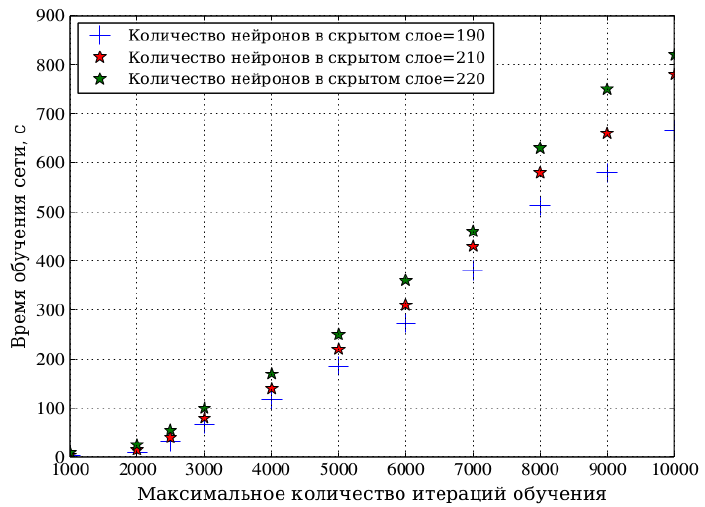
\includegraphics[width=.8\textwidth]{time_from_iter.png}
  \caption{Исследование времени обучения в зависимости от числа максимальных 
итераций обучения нейронной сети.}
  \label{fig:time}
\end{figure}

\subsection*{Выводы}
\addcontentsline{toc}{subsection}{Выводы}

Проведенные эксмперименты показали, что увеличение числа нейронов в сети
приводит к росту времени обучения нейронной сети, однако при большем числе нейронов в скрытом
слое, достоверность распознавания увеличивается.

\clearpage

%	\section*{Заключение} \addcontentsline{toc}{section}{Заключение}

В ходе разработки проекта был изучен набор алгоритмов для распознавания лиц в
реальном времени, изучены новые возможности языка C++ и его подмножества C++11,
изучено и применено несколько сторонних библиотек, отточены навыки
программирования и использования некоторых технических средств. Итогом работы
является целиком завершённая программа, а также некоторый исследовательский
материал на её основе. В целом, работа выполнена успешно.



%	\input{appendix}
	\newpage
    \bibliographystyle{plain}
	%\addcontentsline{toc}{section}{\bibname}
	%\nocite{*}
	%\bibliography{biblio}
\end{document}
